% =====================================================================
% Práctica 2 de Robótica Inteligente Aplicada — memoria
% Compilar con pdfLaTeX (en Overleaf: compilador pdfLaTeX).
% Calibri no está en TeX Live: se usa Carlito, con las mismas métricas.
% =====================================================================
\documentclass[11pt,a4paper]{article}

\usepackage[T1]{fontenc}
\usepackage[utf8]{inputenc}
\usepackage[spanish,es-noshorthands,es-tabla]{babel}
\usepackage[sfdefault,lining]{carlito}
\usepackage[a4paper,top=2.2cm,bottom=2.2cm,left=2.2cm,right=2.2cm]{geometry}
\usepackage{graphicx}
\usepackage{booktabs}
\usepackage{tabularx}
\usepackage{adjustbox}
\usepackage{xcolor}
\usepackage[font=small,labelfont=bf,labelsep=colon,skip=4pt]{caption}
\usepackage{enumitem}
\usepackage[colorlinks,linkcolor=blue,urlcolor=black]{hyperref}

\setlength{\parindent}{0pt}
\setlength{\parskip}{6pt}
\setlist{nosep,leftmargin=*}
\renewcommand{\arraystretch}{1.1}
\graphicspath{{figuras/}}

\newcommand{\grados}{\textdegree}
\newcommand{\code}[1]{\texttt{#1}}
\newcommand{\figref}[1]{\hyperref[#1]{Figura~\ref*{#1}}}

\makeatletter
\renewcommand\section{\@startsection{section}{1}{\z@}{-2ex plus -0.5ex}{1ex}{\normalfont\large\bfseries}}
\renewcommand\subsection{\@startsection{subsection}{2}{\z@}{-1.5ex plus -0.3ex}{0.6ex}{\normalfont\normalsize\bfseries}}
\makeatother

\begin{document}

{\Large\bfseries Práctica 2. Seguimiento de un vehículo en Follow City con neuroevolución}\par
\vspace{4pt}
{\small Robótica Inteligente Aplicada. Grado en Inteligencia Artificial.\\
Jacobo Callejo Iribarren (jacobo.callejo@udc.es) - Francisco Novo Rego (francisco.novo.rego@udc.es)}

% =====================================================================
\section{Introducción}

El objetivo de la práctica es el mismo que en la Práctica 1: que un Robobo, el seguidor, circule detrás del
vehículo guía de Follow City manteniendo la separación con su pelota verde entre 0,20 y 0,45 m, sin chocar, sin
perderlo de vista y sin salirse de su carril, usando solo sus sensores a través de ROS 2. La diferencia está en
cómo se obtiene el controlador. En lugar de entrenar una política por refuerzo, se evoluciona una red neuronal
con NEAT, que ajusta a la vez sus pesos y su topología.

Se han trabajado las cuatro configuraciones del guía: C1 (crucero 10-10), C2 (crucero 10-40), C3 (variable
10-40) y C4 (variable 10-40 con paradas aleatorias). Las tres primeras son las de la P1, lo que permite comparar
las dos técnicas, y la cuarta obliga al seguidor a detenerse detrás del guía y a volver a arrancar con él. Cada
controlador se ha evaluado con el protocolo del anexo B: episodios de 120 s con reinicio de la escena.

% =====================================================================
\section{Archivos y manual de ejecución}

\begin{table}[h]
\centering\small
\caption{Archivos entregados.}
\label{tab:archivos}
\begin{tabularx}{\textwidth}{@{}lX@{}}
\toprule
Archivo & Contenido \\
\midrule
\code{p1\_*.py}, \code{p1\_config.json} & Entorno de Gymnasium, conexión con el simulador, evaluador y calibración de la P1, sin modificar. \\
\code{p2\_neat.py} & Programa principal: evolución, reanudación, reevaluación y ejecución de los controladores. \\
\code{p2\_calidad.py} & Función de calidad. \\
\code{p2\_registro.py} & Registro de cada generación (calidad, especies, coste). \\
\code{p2\_protocolo.py} & Evaluador del anexo B, el de la P1 con C4 añadida. \\
\code{config-p2.ini}, \code{config-p2-v6.ini} & Parámetros de NEAT en sus dos versiones (v5 y v6). \\
\code{p2\_runs/} & Un directorio por evolución con su registro, sus puntos de control y el genoma final. \\
\code{p2\_eval/} & Registro paso a paso de cada episodio de evaluación. \\
\code{videos/} & Un vídeo por configuración con su controlador final evaluándose. \\
\bottomrule
\end{tabularx}
\end{table}

Cada evolución tiene un nombre del tipo \code{C2\_v5\_p235\_s3}, que indica la configuración, la versión de los
parámetros, la duración del episodio si no es la de por defecto y la semilla.

\textbf{Vídeos.} En la carpeta \code{videos} hay un vídeo de cada configuración con su controlador final, grabado
mientras se evaluaba con el protocolo.

Para ejecutar, se abre RoboboSim en Follow City con el guía configurado (C1: Mode 1, 10-10; C2: Mode 1, 10-40;
C3: Mode 2, 10-40; C4: Mode 3, 10-40) y la ventana en primer plano. Dentro del contenedor se lanza en un terminal
el puente solo con el módulo de blobs:

{\small
\begin{verbatim}
  ros2 run robobo_ros2 robobo_container --ros-args -p ip:=host.docker.internal -p modules:="['blob']"
\end{verbatim}
}

y en otro, desde \code{/docker-ros/ws}, se ejecutan los programas en este orden:
\begin{enumerate}
  \item Evolución desde cero: \code{p2\_neat.py --evolucionar --etiqueta C1 --semilla 1 --generaciones 20
        --pasos 150}. Con \code{--desde} se continúa la población de otra evolución, por ejemplo
        {--desde p2\_runs/C1\_v5\_s2/chk/p2-12}, y con {--reanudar} se sigue una evolución cortada.
  \item Elección del controlador final: \code{p2\_neat.py --reevaluar --salida p2\_runs/C1\_v5\_s2}.
  \item Evaluación con el protocolo: \code{p2\_protocolo.py --evaluar --run p2\_runs/C1\_v5\_s2
        --configuracion C1}, o con \code{--manual} y \code{--aleatoria} para la línea base.
  \item Resultados: \code{p2\_protocolo.py p2\_eval/*.csv} genera las tablas y \code{p2\_figuras.py}, las curvas.
\end{enumerate}

% =====================================================================
\section{Diseño}

El controlador es una red neuronal que, en cada paso, recibe lo que miden los sensores del seguidor y devuelve
la velocidad con la que tiene que moverse. Se ha reutilizado todo el entorno de la P1 (la comunicación con ROS 2,
la calibración y el paso de control), así que el diseño de esta práctica se reduce a tres decisiones: qué recibe
la red, cómo es la red y cómo se evalúa cada individuo durante la evolución.

\subsection{Entradas y salidas de la red}

La observación de la P1 tenía 11 valores. Para la red se han dejado los 6 de la Tabla \ref{tab:entradas}, que
son los que hacen falta para seguir al guía, y se han transformado para que, cuando el seguimiento es bueno,
casi todos valgan cero y el resto sean pequeños. El motivo es que NEAT empieza con redes de pesos aleatorios: si las entradas son
grandes, la salida de esas redes queda saturada en uno de sus extremos y el robot solo sabe ir a tope o
quedarse quieto. Con entradas cercanas a cero, una red nueva responde de forma suave y la evolución tiene algo
que mejorar desde el principio.

\begin{table}[h]
\centering\small
\caption{Entradas de la red. Todas salen de los sensores del seguidor.}
\label{tab:entradas}
\begin{tabularx}{\textwidth}{@{}lXl@{}}
\toprule
Entrada & Qué mide & Vale cero cuando \\
\midrule
Error de distancia & Distancia a la pelota respecto al centro de la banda (0,325 m) & Está en el centro de la banda \\
Posición de la pelota & Posición horizontal del blob en la imagen & La pelota está centrada \\
Cambio de distancia & Si la pelota se aleja o se acerca & Va a la misma velocidad que el guía \\
Velocidad del guía & Estimación a partir de la velocidad propia y del cambio de distancia & El guía está parado \\
Tiempo sin pelota & Segundos desde que se dejó de ver, divididos entre 3 & Ve la pelota \\
Infrarrojo frontal & Proximidad de un obstáculo delante & No hay nada cerca \\
\bottomrule
\end{tabularx}
\end{table}

La distancia se estima por el tamaño del blob, igual que en la P1, pero con una corrección. Cuando el seguidor
está muy cerca, la pelota se corta por el borde inferior de la imagen, el blob parece más pequeño y la distancia
estimada salta de golpe hacia arriba. Una red que se fiara de esa lectura aceleraría justo cuando está a punto
de chocar, así que, si la distancia sube de forma imposible en un solo paso, se considera que el seguidor está
pegado al guía.

Las salidas son las mismas que en la P1: la velocidad lineal, entre 0 y 0,35 m/s, y la velocidad angular, entre
-0,6 y 0,6 rad/s. Cada paso de control dura alrededor de medio segundo.

\subsection{La red y los parámetros de NEAT}

Al empezar, la red es lo más sencilla posible: las 6 entradas conectadas directamente a las 2 salidas, sin
neuronas ocultas. A partir de ahí es la evolución la que añade o quita conexiones y neuronas. La activación es
la tangente hiperbólica, que da valores entre -1 y 1 y se reescala al rango de cada salida.

Se partió de los parámetros de las indicaciones técnicas y solo se cambiaron los que dieron problemas
(Tabla \ref{tab:neat}). Con una población de 20 individuos, el umbral de compatibilidad original dejaba muy pocas
especies, así que se bajó para que las innovaciones quedaran protegidas en especies propias. El estancamiento se
alargó y se protegieron dos especies, porque con una calidad tan ruidosa una especie buena podía parecer
estancada y desaparecer. Los sesgos iniciales se redujeron por el mismo motivo que las entradas, para no
saturar las salidas. Más adelante se vio que la mutación de los pesos era demasiado fuerte y se creó la versión
v6, que solo se diferencia de la v5 en que muta menos los pesos y los sesgos.

\begin{table}[h]
\centering\small
\caption{Parámetros de NEAT. Solo se indican los que cambian respecto a las indicaciones técnicas.}
\label{tab:neat}
\begin{tabular}{@{}lccc@{}}
\toprule
Parámetro & Indicaciones & v5 & v6 \\
\midrule
Umbral de compatibilidad & 3,0 & 1,3 & 1,3 \\
Estancamiento máximo & 8 & 20 & 20 \\
Especies protegidas & 1 & 2 & 2 \\
Dispersión inicial de los sesgos & 1,0 & 0,3 & 0,3 \\
Potencia de mutación de los sesgos & 0,5 & 0,3 & 0,15 \\
Probabilidad de mutar un peso & 0,8 & 0,8 & 0,5 \\
Potencia de mutación de los pesos & 0,5 & 0,5 & 0,2 \\
Probabilidad de reemplazar un peso & 0,1 & 0,1 & 0,02 \\
\bottomrule
\end{tabular}
\end{table}

\subsection{Evaluación de cada individuo}

Para saber lo bueno que es un individuo, su red conduce al seguidor durante un episodio, o dos en C4, y de ese
episodio sale su calidad (apartado \ref{sec:calidad}). Cada episodio empieza con un reinicio de la escena, igual
que en el protocolo, para que todos los individuos de una generación partan de la misma situación y se puedan
comparar entre sí. El episodio dura 150 pasos (unos 77 s) en C1 y C4, y 235 pasos (los 120 s del protocolo) en
C2 y C3; el motivo de esta diferencia se explica en el apartado de C2. Además de los fallos del protocolo, el
episodio termina si el seguidor se sale de la calzada o adelanta al guía.

Como una evolución dura varias horas, en cada generación se guarda un punto de control desde el que se puede
reanudar si algo falla. Además, cada cinco generaciones se ejecuta el controlador programado a mano: si deja de
completar el episodio, el simulador se ha degradado y la evolución se detiene antes de estropear la población.

Por último, la calidad de un solo episodio es muy ruidosa, así que el controlador final no es el mejor de la
última generación. Al terminar la evolución se vuelven a evaluar con tres episodios los mejores genomas
registrados y se elige el que completa más episodios.

% =====================================================================
\section{Función de calidad}\label{sec:calidad}

La calidad se calcula en \code{p2\_calidad.py}. A diferencia de la recompensa de la P1, puede usar información
del simulador que el robot no tiene, porque solo sirve para comparar individuos y la red nunca la recibe. Se
usan la separación real con la pelota, el ángulo real de la pelota y la distancia del seguidor a la línea
central de su carril.

En cada paso se calculan tres notas entre 0 y 1:
\begin{itemize}
  \item Nota de separación: vale 1 dentro de la banda de 0,20 a 0,45 m y baja hasta 0 en la distancia de choque
        (0,12 m) y en la de pérdida (0,90 m).
  \item Nota de orientación: vale 1 si la pelota está a menos de 15 grados del centro y baja hasta 0 en el borde
        de la imagen, a unos 23 grados.
  \item Nota de carril: vale 1 si el robot cabe entero en su carril y baja hasta 0 cuando su centro pisa la raya.
\end{itemize}
La nota del paso es el producto de las tres, para que un paso solo puntúe alto si se cumplen los tres requisitos
a la vez.

La calidad del episodio va de 0 a 100 y tiene tres partes. Hasta 20 puntos se dan por la parte del episodio que
el seguidor sobrevive, hasta 70 por la media de la nota de cada paso y 10 más si completa el episodio. La parte
de supervivencia es la que permite distinguir, desde la primera generación, entre redes malas y menos malas,
cuando todavía ninguna sabe seguir al guía. Como referencia, el controlador programado a mano obtiene 96,4 en
C1 y 90,1 en C3.

% =====================================================================
\section{Resultados por configuración}

Las configuraciones se han resuelto de forma incremental: cada evolución parte de la población guardada de la
anterior, con sus pesos, sus topologías y sus especies. Las curvas de evolución están en la \figref{fig:evol},
la especiación en la \figref{fig:especies}, los episodios completados en la \figref{fig:completados} y las redes
elegidas en la \figref{fig:redes}. En todas las evoluciones la población es de 20 individuos.

En las tablas, la columna Reeval. indica los episodios completados de 3 al volver a evaluar el genoma final, y
Calidad, su calidad media en esos episodios.

\subsection{C1: crucero 10-10}

C1 se evolucionó desde cero con tres semillas y la versión v5, y después se repitió la semilla 3 con la v6.

\begin{table}[h]
\centering\small
\caption{C1. Evolución y evaluación con el protocolo (episodios de 120 s).}
\label{tab:c1}
\begin{adjustbox}{max width=\textwidth}
\begin{tabular}{@{}lrrrcrcrrrr@{}}
\toprule
& \multicolumn{5}{c}{Evolución} & \multicolumn{5}{c}{Evaluación} \\
\cmidrule(lr){2-6}\cmidrule(l){7-11}
Controlador & Gen. & Pasos & Horas & Reeval. & Calidad & Compl. & En banda & Sep. media & Desv. media & En carril \\
\midrule
Aleatoria & & & & & & 0/3 & 40,0 \% & 0,195 m & 16,0\grados & 100 \% \\
A mano & & & & 3/3 & 96,4 & & & & & \\
NEAT v5 s1 & 20 & 7340 & 2,1 & 1/3 & 29,1 & 2/2 & 99,8 \% & 0,332 m & 6,4\grados & 98,7 \% \\
\textbf{NEAT v5 s2} & 20 & 13218 & 2,6 & \textbf{3/3} & 93,0 & \textbf{2/2} & \textbf{100 \%} & 0,326 m & 7,9\grados & 100 \% \\
NEAT v5 s3 & 20 & 11482 & 2,4 & 0/3 & 18,8 & 0/1 & 86,8 \% & 0,398 m & 13,4\grados & 100 \% \\
NEAT v6 s3 & 15 & 19265 & 3,3 & 3/3 & 95,9 & 1/1 & 100 \% & 0,318 m & 4,9\grados & 100 \% \\
\bottomrule
\end{tabular}
\end{adjustbox}
\end{table}

Con la v5, el mejor individuo de cada semilla llega a superar 90, pero la media de la población apenas pasa de 20
(\figref{fig:evol}). Hay dos motivos. El primero es el ruido: un mismo genoma puede sacar 24 en un episodio y 93
en el siguiente, de modo que la selección premia la suerte. El segundo es que la mutación era demasiado fuerte y
los hijos de buenos padres salían mucho peores. Al reevaluar, solo la semilla 2 da un genoma que completa los tres
episodios. Con la v6, que muta menos, la población mejora mucho y llega a completar más de la mitad de los
episodios de una generación, pero se queda con una sola especie (\figref{fig:especies}).

La red elegida se parece al controlador a mano: acelera cuando la pelota se aleja y gira hacia el lado en que la
ve. Además, cuando pierde la pelota gira con fuerza hacia la izquierda. Como el circuito gira siempre a la
izquierda, la pelota se pierde por el interior de las curvas, y la evolución ha aprovechado esa regularidad.

\textbf{Controlador elegido: genoma 160 (v5 s2).} Completa los tres episodios de la reevaluación y los dos del
protocolo sin salir nunca de la banda.

\subsection{C2: crucero 10-40}

C2 se evolucionó a partir de la población de C1 v5 s2 en la generación 12.

\begin{table}[h]
\centering\small
\caption{C2. Evolución y evaluación con el protocolo (episodios de 120 s).}
\label{tab:c2}
\begin{adjustbox}{max width=\textwidth}
\begin{tabular}{@{}lrrrcrcrrrr@{}}
\toprule
& \multicolumn{5}{c}{Evolución} & \multicolumn{5}{c}{Evaluación} \\
\cmidrule(lr){2-6}\cmidrule(l){7-11}
Controlador & Gen. & Pasos & Horas & Reeval. & Calidad & Compl. & En banda & Sep. media & Desv. media & En carril \\
\midrule
Aleatoria & & & & & & 0/1 & 100 \% & 0,360 m & 21,3\grados & 73,7 \% \\
A mano & & & & & & 1/1 & 41,9 \% & 0,456 m & 3,2\grados & 100 \% \\
NEAT s2, 150 pasos & 30 & 11137 & 2,7 & 1/3 & 40,8 & 0/3 & 68,1 \% & 0,434 m & 35,3\grados & 86,1 \% \\
NEAT s1, 235 pasos & 25 & 9225 & 2,3 & 0/3 & 12,5 & 0/1 & 37,5 \% & 0,482 m & 23,1\grados & 100 \% \\
\textbf{NEAT s3, 235 pasos} & 21 & 15724 & 3,1 & \textbf{3/3} & 84,9 & 0/1 & \textbf{91,4 \%} & 0,352 m & 6,5\grados & 100 \% \\
\bottomrule
\end{tabular}
\end{adjustbox}
\end{table}

El primer intento, con episodios de 150 pasos, no funcionó: el mejor genoma completaba uno de cada tres
episodios y en el protocolo perdía la pelota en los primeros segundos. La razón es que 150 pasos no llegan al
tramo en el que el guía acelera hasta 40 y luego frena en la curva, así que la evolución nunca veía la situación
en la que fallaba. Al alargar los episodios a 235 pasos, la semilla 3 encontró en la generación 12 el genoma
411, que desde ese momento completó todos sus episodios de evolución y los tres de la reevaluación. La semilla 1
se estancó.

El genoma 411 es una red de solo 9 parámetros y se puede leer casi como un controlador hecho a mano. La
velocidad aumenta con el error de distancia, de modo que el seguidor se queda a la distancia en la que va tan
rápido como el guía. El giro sigue a la pelota con una ganancia parecida a la del controlador a mano. Si pierde
la pelota, frena y gira hacia el interior de la curva, y en las curvas reduce algo la velocidad. Tiene, sin
embargo, un defecto: el infrarrojo frontal le hace acelerar. Como en C1, C2 y C3 el infrarrojo casi nunca se
activa, la evolución no lo ha castigado, y eso es lo que ocurrió en el protocolo. Durante 35 s siguió al guía
dentro de la banda el 91 \% del tiempo, pero el guía frenó en seco, el seguidor no redujo la velocidad y chocó.

\textbf{Controlador elegido: genoma 411 (s3).} Es el único que completa los tres episodios de la reevaluación,
aunque en el episodio del protocolo chocó tras una frenada brusca del guía.

\subsection{C3: variable 10-40}

C3 se evolucionó con dos semillas a partir de la población de C2 s3 en la generación 18, en la que seguía el
genoma 411. Antes se había intentado pasar directamente de C1 a C3 con la v6.

\begin{table}[h]
\centering\small
\caption{C3. Evolución y evaluación con el protocolo (episodios de 120 s).}
\label{tab:c3}
\begin{adjustbox}{max width=\textwidth}
\begin{tabular}{@{}lrrrcrcrrrr@{}}
\toprule
& \multicolumn{5}{c}{Evolución} & \multicolumn{5}{c}{Evaluación} \\
\cmidrule(lr){2-6}\cmidrule(l){7-11}
Controlador & Gen. & Pasos & Horas & Reeval. & Calidad & Compl. & En banda & Sep. media & Desv. media & En carril \\
\midrule
Aleatoria & & & & & & 0/1 & 80,0 \% & 0,289 m & 37,5\grados & 100 \% \\
A mano & & & & 3/3 & 90,1 & 1/1 & 49,6 \% & 0,455 m & 3,2\grados & 100 \% \\
\textbf{NEAT v5 s1} & 10 & 8609 & 1,6 & \textbf{3/3} & 83,5 & \textbf{1/1} & \textbf{97,9 \%} & 0,351 m & 6,9\grados & 97,0 \% \\
NEAT v5 s2 & 10 & 9714 & 1,8 & 2/3 & 78,7 & 1/1 & 95,3 \% & 0,356 m & 6,3\grados & 99,6 \% \\
NEAT v6 s1, desde C1 & 10 & 6926 & 1,4 & 0/3 & 15,8 & & & & & \\
NEAT v6 s2, desde C1 & 10 & 4541 & 1,1 & 0/3 & 18,6 & & & & & \\
NEAT v6 s3, desde C1 & 10 & 2620 & 0,9 & 0/3 & 17,5 & & & & & \\
\bottomrule
\end{tabular}
\end{adjustbox}
\end{table}

Partiendo de C2, desde la primera generación ya hay individuos que completan los episodios, es decir, el
controlador de C2 se adapta bien al modo variable. El 411 completa casi siempre, aunque a veces choca cuando el
guía frena fuerte y entonces la población lo pierde. Durante la evolución aparecen genomas nuevos que también
completan varias generaciones seguidas, pero al reevaluar el mejor sigue siendo el 411 en las dos semillas. En
el protocolo completa los dos episodios y pasa casi todo el tiempo en la banda, mientras que el controlador a
mano va más lejos, aunque más centrado (\figref{fig:traza}).

El intento de pasar directamente de C1 a C3 fracasó en las tres semillas. La población de C1, con un guía a
velocidad constante, nunca había necesitado usar la velocidad del guía, y con la v6 había una sola especie.
Pasar por C2 es lo que hace funcionar la evolución incremental. También es llamativo que un genoma evolucionado
solo en C1 (v5 s1) completara dos episodios del protocolo de C3.

\textbf{Controlador elegido: genoma 411.} El mismo que en C2: completa los tres episodios de la reevaluación y
los dos del protocolo.

\subsection{C4: variable 10-40 con paradas}

C4 se evolucionó con tres semillas a partir de la población de C3 v6 en la generación 4, con dos episodios por
individuo para suavizar el azar de las paradas.

\begin{table}[h]
\centering\small
\caption{C4. Evolución (dos episodios por individuo) y evaluación con el protocolo (dos episodios de 120 s).}
\label{tab:c4}
\begin{adjustbox}{max width=\textwidth}
\begin{tabular}{@{}lrrrcrcrrrr@{}}
\toprule
& \multicolumn{5}{c}{Evolución} & \multicolumn{5}{c}{Evaluación} \\
\cmidrule(lr){2-6}\cmidrule(l){7-11}
Controlador & Gen. & Pasos & Horas & Reeval. & Calidad & Compl. & En banda & Sep. media & Desv. media & Paradas \\
\midrule
\textbf{NEAT v6 s1} & 10 & 15388 & 3,0 & \textbf{2/3} & 79,6 & & & & & \\
NEAT v6 s2 & 10 & 7575 & 2,0 & 1/3 & 45,8 & & & & & \\
NEAT v6 s3 & 10 & 11943 & 2,3 & & & & & & & \\
\bottomrule
\end{tabular}
\end{adjustbox}
\end{table}

En la semilla 1, los episodios completados suben hasta una cuarta parte de la población en la generación 4 y
después caen a cero. Coincide con que la v6 deja una sola especie, de modo que cuando la especie empeora no hay
otra que la sustituya. La red obtenida corrige el defecto del 411: aquí el infrarrojo frontal frena con fuerza,
que es justo lo que hace falta para detenerse detrás de un guía parado.

\textbf{Controlador elegido: genoma 446 (v6 s1).} Es el que más episodios completa en la reevaluación.

% =====================================================================
\section{Comparación con la Práctica 1}

\begin{table}[h]
\centering\small
\caption{Controlador final de la P1 (SAC) y de la P2 (NEAT) en cada configuración. En NEAT, los pasos y las horas
son los de las evoluciones necesarias hasta obtener el genoma.}
\label{tab:p1}
\begin{tabular}{@{}llcrrrrr@{}}
\toprule
Conf. & Controlador & Compl. & En banda & Desv. media & Pasos & Horas & Parámetros \\
\midrule
C1 & SAC s0 & 3/3 & 100 \% & 2,1\grados & 9431 & 1,7 & 69892 \\
C1 & NEAT 160 & 2/2 & 100 \% & 7,9\grados & 13218 & 2,6 & 14 \\
\midrule
C2 & SAC s1 & 3/3 & 98,2 \% & 4,6\grados & 12550 & 2,0 & 69892 \\
C2 & NEAT 411 & 0/1 & 91,4 \% & 6,5\grados & 13086 & 2,8 & 9 \\
\midrule
C3 & SAC s0 & 0/1 & 72,1 \% & 12,8\grados & 8337 & 1,4 & 69892 \\
C3 & NEAT 411 & 2/2 & 96,6 \% & 6,6\grados & 13086 & 2,8 & 9 \\
\bottomrule
\end{tabular}
\end{table}

En C1 y C2, SAC es más preciso: completa más episodios y centra mucho mejor la pelota. Es lógico, porque recibe
una recompensa en cada paso, mientras que NEAT solo recibe una calidad por episodio. En C3 ocurre lo contrario:
ninguna semilla de SAC completó C3, y el 411 lo completa con más tiempo en la banda (Tabla \ref{tab:p1}). El coste
de obtener cada controlador es parecido, entre una hora y media y tres horas de simulación, aunque en NEAT la mayor
parte del tiempo se va en reiniciar la escena para cada individuo. La gran diferencia está en el tamaño: el actor
de SAC tiene casi 70000 parámetros y el 411 tiene 9. Por eso la red evolucionada se puede interpretar conexión a
conexión, y eso es lo que nos ha permitido encontrar la causa de la colisión en C2.

% =====================================================================
\section{Conclusiones}

En este problema, el aprendizaje por refuerzo ha dado controladores más finos, y la neuroevolución,
controladores mucho más pequeños, fáciles de entender y que generalizan mejor entre configuraciones: el 411, con
nueve parámetros, sigue al guía tanto en C2 como en C3. El principal inconveniente de NEAT es el ruido. Como
cada individuo recibe una única calidad por episodio, una red buena puede tener un mal episodio y desaparecer de
la población, y por eso ha sido imprescindible reevaluar antes de elegir. También ha sido clave la evolución
incremental, ya que saltarse C2 hizo fracasar C3.

Por el camino aparecieron varios problemas que hubo que resolver: una sesión en la que la posición de la pelota
llegaba invertida, la degradación del simulador en sesiones largas, un fallo de NEAT-Python al recuperar los
puntos de control, episodios demasiado cortos para C2 y una mutación excesiva en la primera versión. Sumando
todas las evoluciones, la práctica ha costado unas 46 horas de simulación. Como mejora, evaluaríamos cada
individuo en varias configuraciones a la vez para obtener un único controlador para todas, y ajustaríamos el
umbral de compatibilidad para que la v6 no se quede con una sola especie.

% =====================================================================
\clearpage
\appendix
\renewcommand{\thefigure}{A\arabic{figure}}
\setcounter{figure}{0}
\section*{Anexo: figuras}


\begin{figure}[h]
\centering
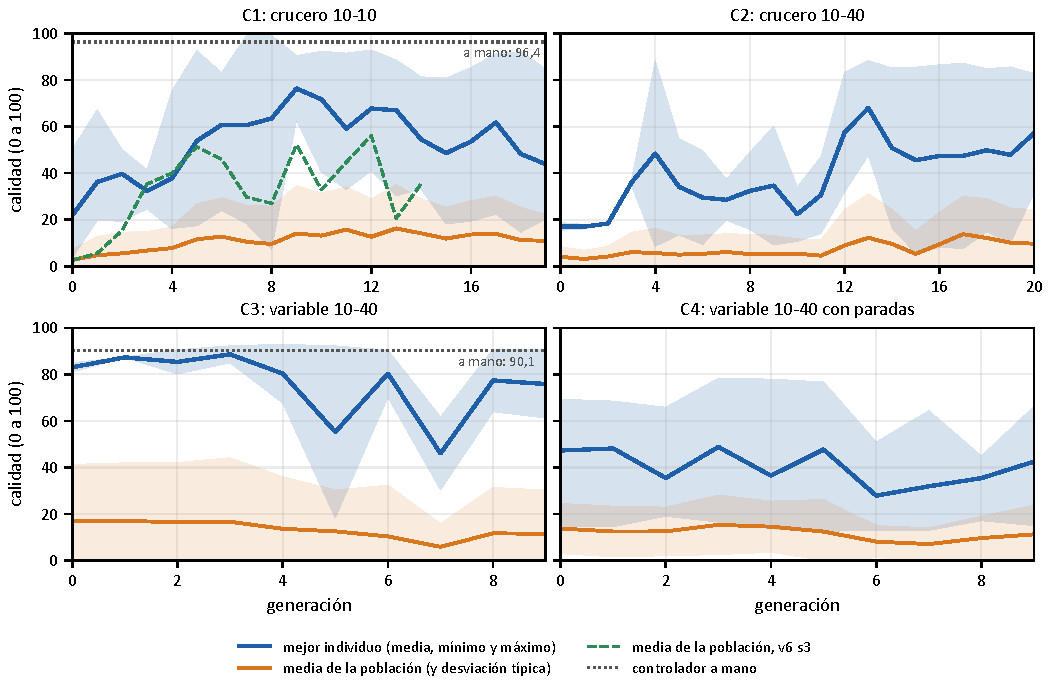
\includegraphics[width=\textwidth]{evolucion.pdf}
\caption{Calidad del mejor individuo (azul) y media de la población (naranja) en cada generación, frente al
controlador a mano (punteado). El coste de cada evolución está en las Tablas \ref{tab:c1} a \ref{tab:c4}.}
\label{fig:evol}
\end{figure}

\begin{figure}[h]
\centering
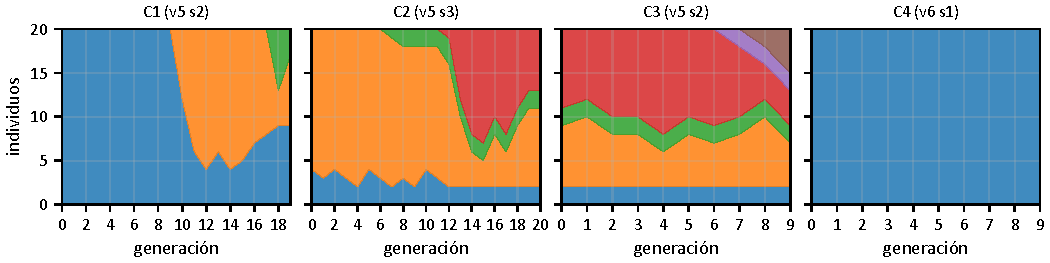
\includegraphics[width=\textwidth]{especies.pdf}
\caption{Individuos de cada especie (un color por especie) a lo largo de una evolución de cada configuración.}
\label{fig:especies}
\end{figure}

\begin{figure}[h]
\centering
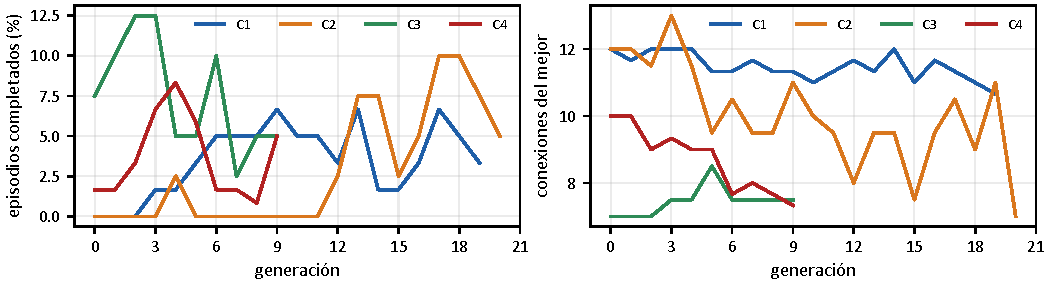
\includegraphics[width=\textwidth]{completados.pdf}
\caption{Episodios completados y conexiones del mejor individuo en cada generación.}
\label{fig:completados}
\end{figure}

\begin{figure}[h]
\centering
\begin{minipage}[b]{0.34\textwidth}\centering
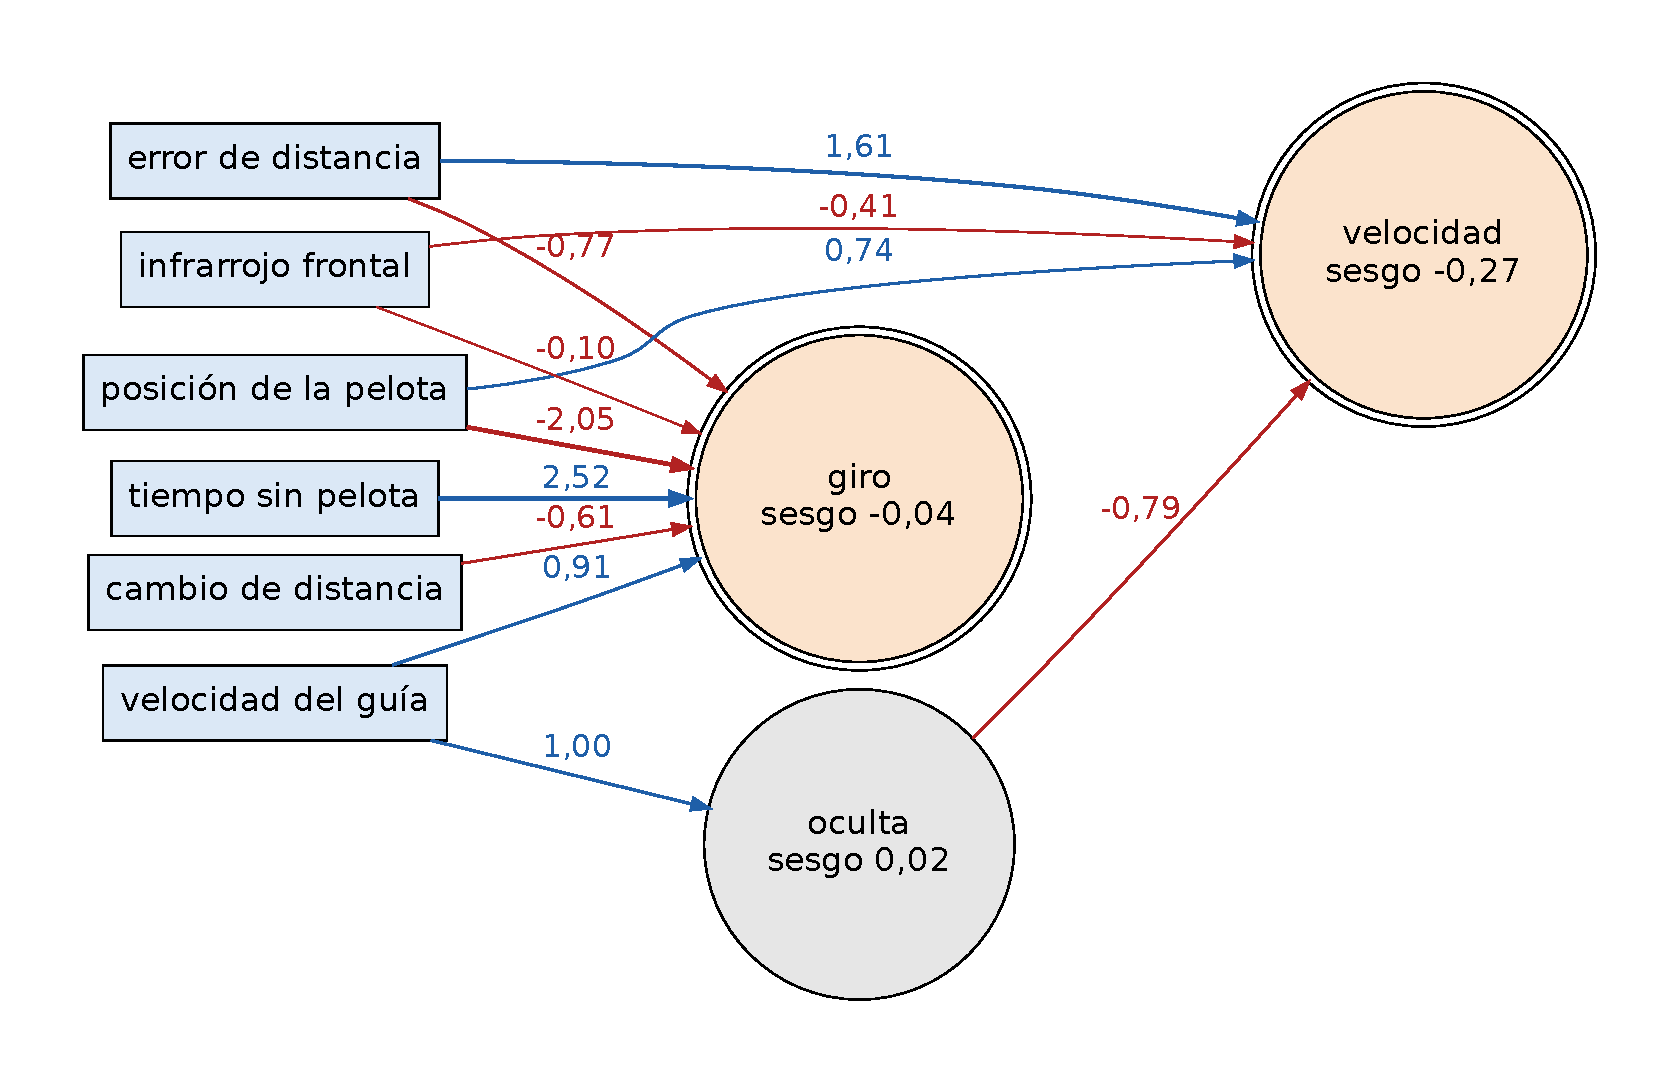
\includegraphics[width=\linewidth]{red_160.pdf}\\{\small Genoma 160 (C1)}
\end{minipage}\hfill
\begin{minipage}[b]{0.31\textwidth}\centering
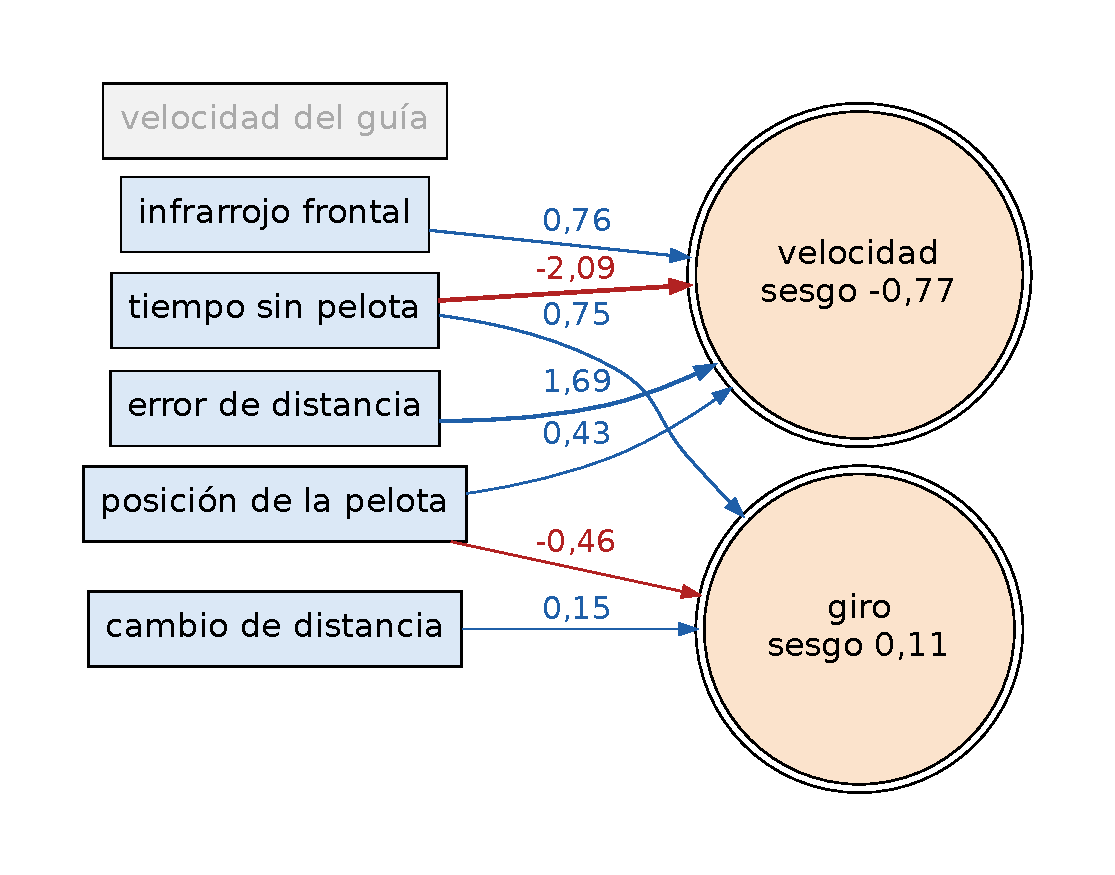
\includegraphics[width=\linewidth]{red_411.pdf}\\{\small Genoma 411 (C2 y C3)}
\end{minipage}\hfill
\begin{minipage}[b]{0.31\textwidth}\centering
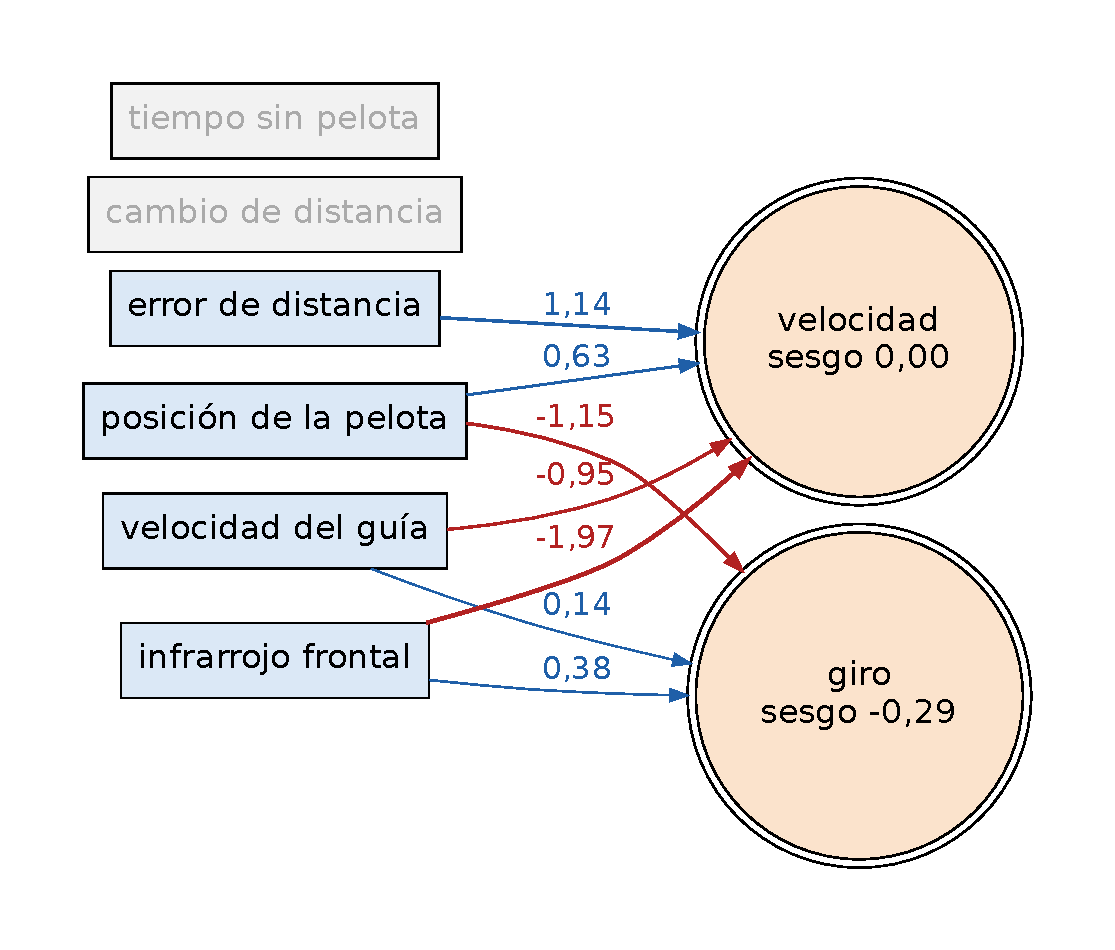
\includegraphics[width=\linewidth]{red_446.pdf}\\{\small Genoma 446 (C4)}
\end{minipage}
\caption{Redes elegidas: conexiones positivas en azul y negativas en rojo, más gruesas cuanto mayor es el peso.}
\label{fig:redes}
\end{figure}

\begin{figure}[h]
\centering
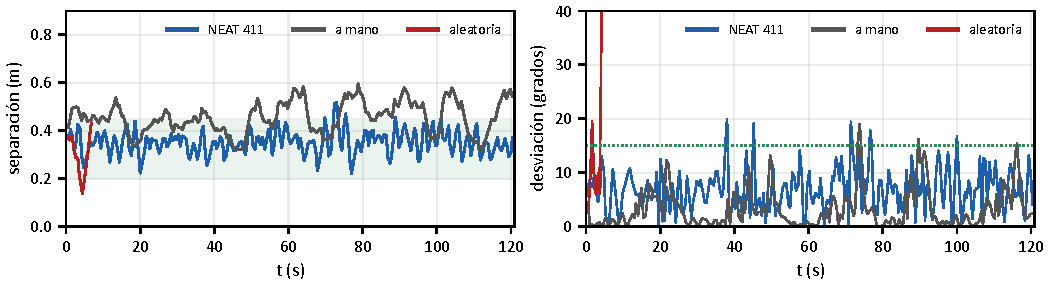
\includegraphics[width=\textwidth]{traza_C3.pdf}
\caption{Separación y desviación durante la evaluación en C3 del genoma 411, el controlador a mano y la política
aleatoria.}
\label{fig:traza}
\end{figure}

\end{document}
